%%%%%%%%%%%%%%%%%%%%%%%%%%%%%%%%%%%%%%%%%%%%%%%%%%%%%%%%%%%%%%%%%%%%%%%
%
%   Presentation of Beamer UNL Theme
%   Beamer Presentation by Chris Bourke
%
%%%%%%%%%%%%%%%%%%%%%%%%%%%%%%%%%%%%%%%%%%%%%%%%%%%%%%%%%%%%%%%%%%%%%%%

\documentclass{beamer}

\usetheme[hideothersubsections]{UNLTheme}
\usepackage[postscript]{ucs}
\usepackage[utf8x]{inputenc}

\title{Performance Modeling and
Design of Computer Systems- Ch 4 \\
Generating Random Variables
for Simulation
}
\author{Debobroto Das Robin} %
\institute{Kent State University}
\date{Spring 2020}




\begin{document}

%{% open a Local TeX Group
%\setbeamertemplate{sidebar}{}
\begin{frame}
        \titlepage
        \begin{center}
    \href{mailto:drobin@kent.edu}{\color{blue}{\texttt{drobin@kent.edu}}}
        \end{center}
\end{frame}

\begin{frame}
\frametitle{Overview} % Table of contents slide, comment this block out to remove it
\tableofcontents % Throughout your presentation, if you choose to use \section{} and \subsection{} commands, these will automatically be printed on this slide as an overview of your presentation
\end{frame}



\section{Introduction}



\begin{frame}
    \frametitle{Random Variable Generation}
    \framesubtitle{\textbf{\textit{}}}
	\begin{itemize}
	
		\item \textbf{Problem} : Assume a system in which  
			\begin{itemize}
			\item \textbf{interarrival times of jobs }are well modeled by an
						\textbf{Exponential distribution } 
			\item \textbf{Job sizes} (service requirements) are well modeled
					by a \textbf{Normal distribution}.
			\item We want to simulate the system 
			\end{itemize}
		\item We need to be able to generate instances of 
			\begin{itemize}
			\item \textbf{Exponential distribution }  \&
			\item \textbf{Job sizes} (service requirements) are well modeled
				\textbf{Normal distribution}.
			\end{itemize}
		\item \textbf{Solution } : 2 Basic maethods for generating random 						variables
			\begin{itemize}
			\item Assuming we already have a generator of Uniform(0,1) random 					variables 
			
			\end{itemize}
		  
	\end{itemize}	    
    
\end{frame}

\section{Inverse-Transform Method}


\begin{frame}
    \frametitle{Inverse-Transform Method}
    \framesubtitle{Basics}
	\begin{itemize}
		\item This method assumes that we know the
		\begin{itemize}
		\item c.d.f. (cumulative distribution function), $F_X (x) = P { X \leq 				x}$, of the random variable $X$ that we are trying to generate, and
		\item that this distribution is easily invertible, namely that we can 				get $x$ from $F_X (x)$
		\end{itemize}
		\item Two variations
		\begin{itemize}
		\item Continuous
		\item Discrete
		\end{itemize}
		
		  
	\end{itemize}	

\end{frame}


\begin{frame}
    \frametitle{Inverse-Transform Method}
    \framesubtitle{Continuous Case}
    \textbf{Idea}: Map each element $u$ generated by uniform distribution to some x of desired distribution
	\begin{itemize}
		\item This method assumes that we know the
		\begin{itemize}
		\item c.d.f. (cumulative distribution function), $F_X (x) = P { X \leq 				x}$, of the random variable $X$ that we are trying to generate, and
		\item that this distribution is easily invertible, namely that we can 				get $x$ from $F_X (x)$
		\end{itemize}
		\item T variations
		\begin{itemize}
		\item Continuous
		\item Discrete
		\end{itemize}
		
		  
	\end{itemize}	

\end{frame}




\begin{frame}
    \frametitle{Inverse-Transform Method}
    \framesubtitle{Basics}
	\begin{itemize}
		\item Server $i$ receives external arrivals (“outside arrivals”) with rate $r_i$ .
		\item Server i also receives internal arrivals from some of the other servers. 
		\item A packet that finishes service at server $i$ is next routed to server $j$ with 							probability $p_{ij}$ . 
		\item Multiple \textbf{“class”} of the packet, may have different probability according to 			routing scheme
%		 \begin{figure}
%        		\begin{center}
%		            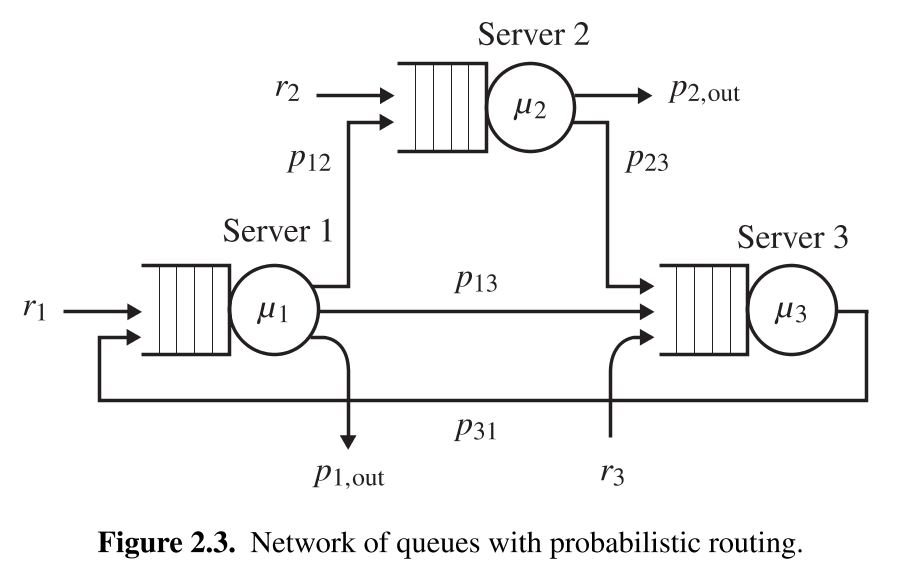
\includegraphics[scale=0.2]{images/Networkqueueswithprobabilisticrouting.jpg}
%					%\caption{Sample caption.}
%        		\end{center}
%		    \end{figure}
		  
	\end{itemize}	    
    
\end{frame}


    
\end{document}